\subsection*{Appendix A - Maxpool positions for TCRs with NLV specificity}

\begin{figure}[H]
\centering
\begin{subfigure}[b]{0.65\textwidth}
   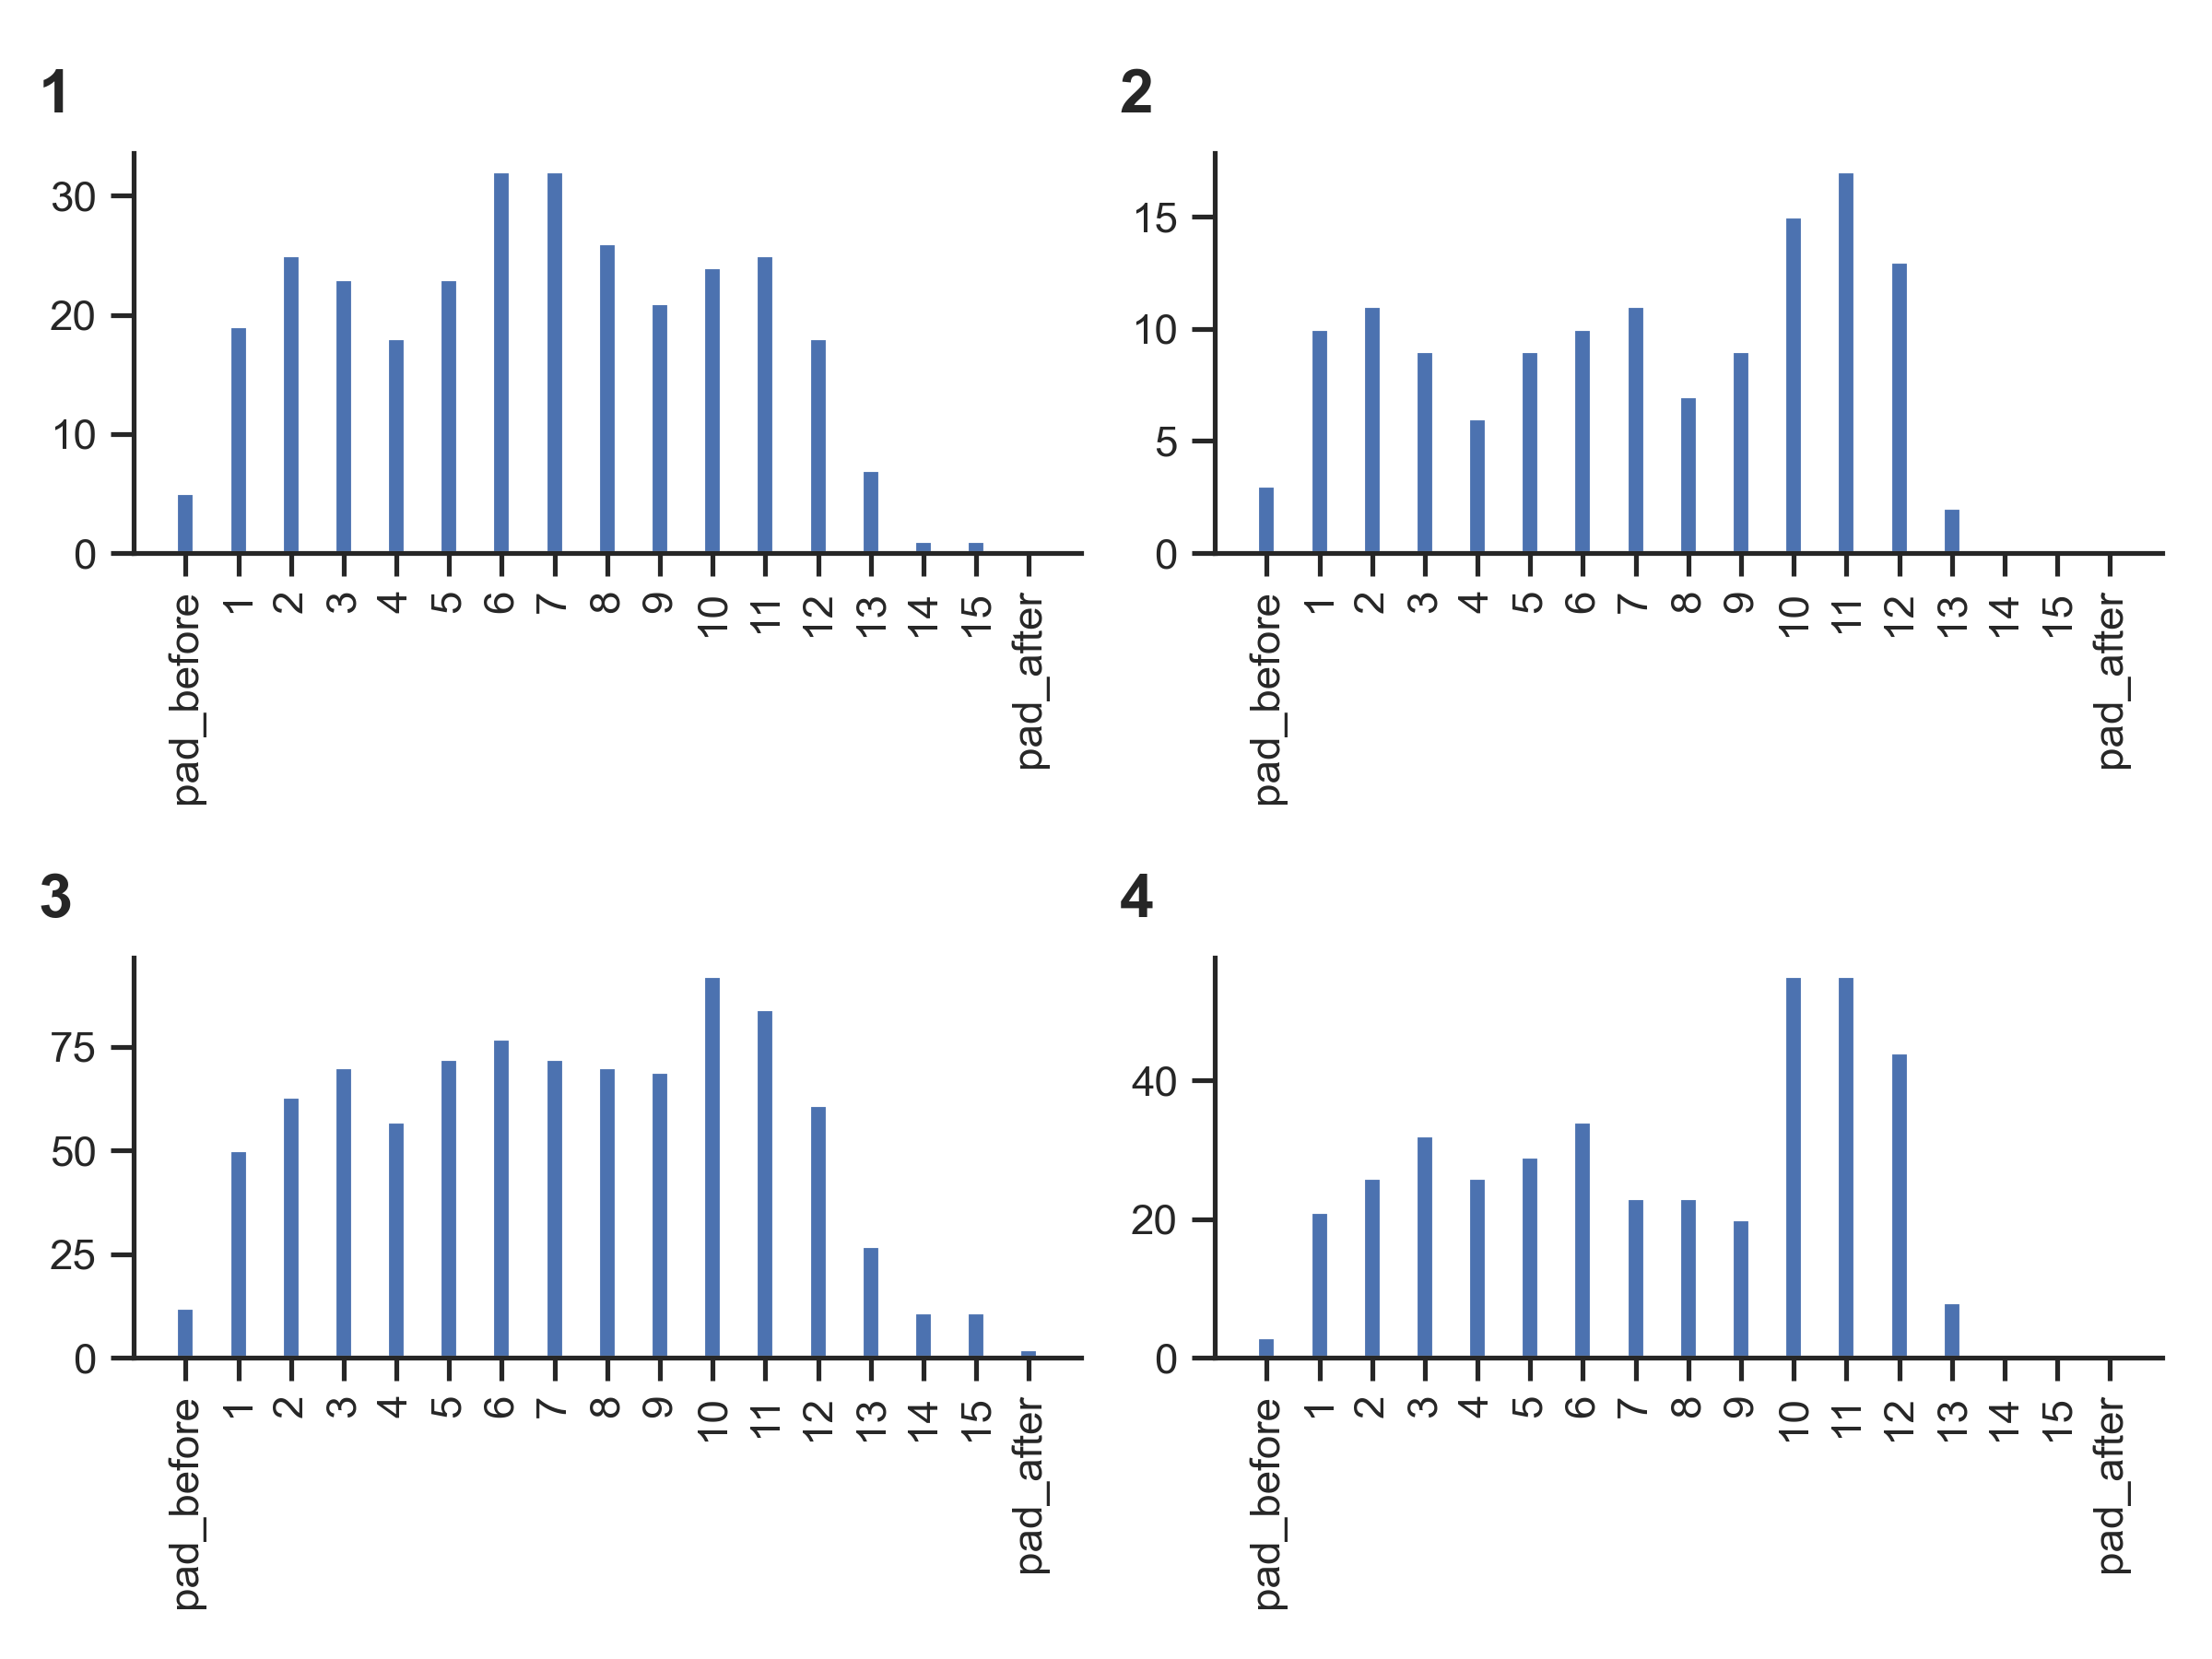
\includegraphics[width=0.95\linewidth]{figures/attention_results/maxpool_cdr3a_nlv12.png}
   \caption{Histograms for CDR3{\textalpha}.}
   \label{fig:pool_nlv12a} 
\end{subfigure}

\begin{subfigure}[b]{0.65\textwidth}
   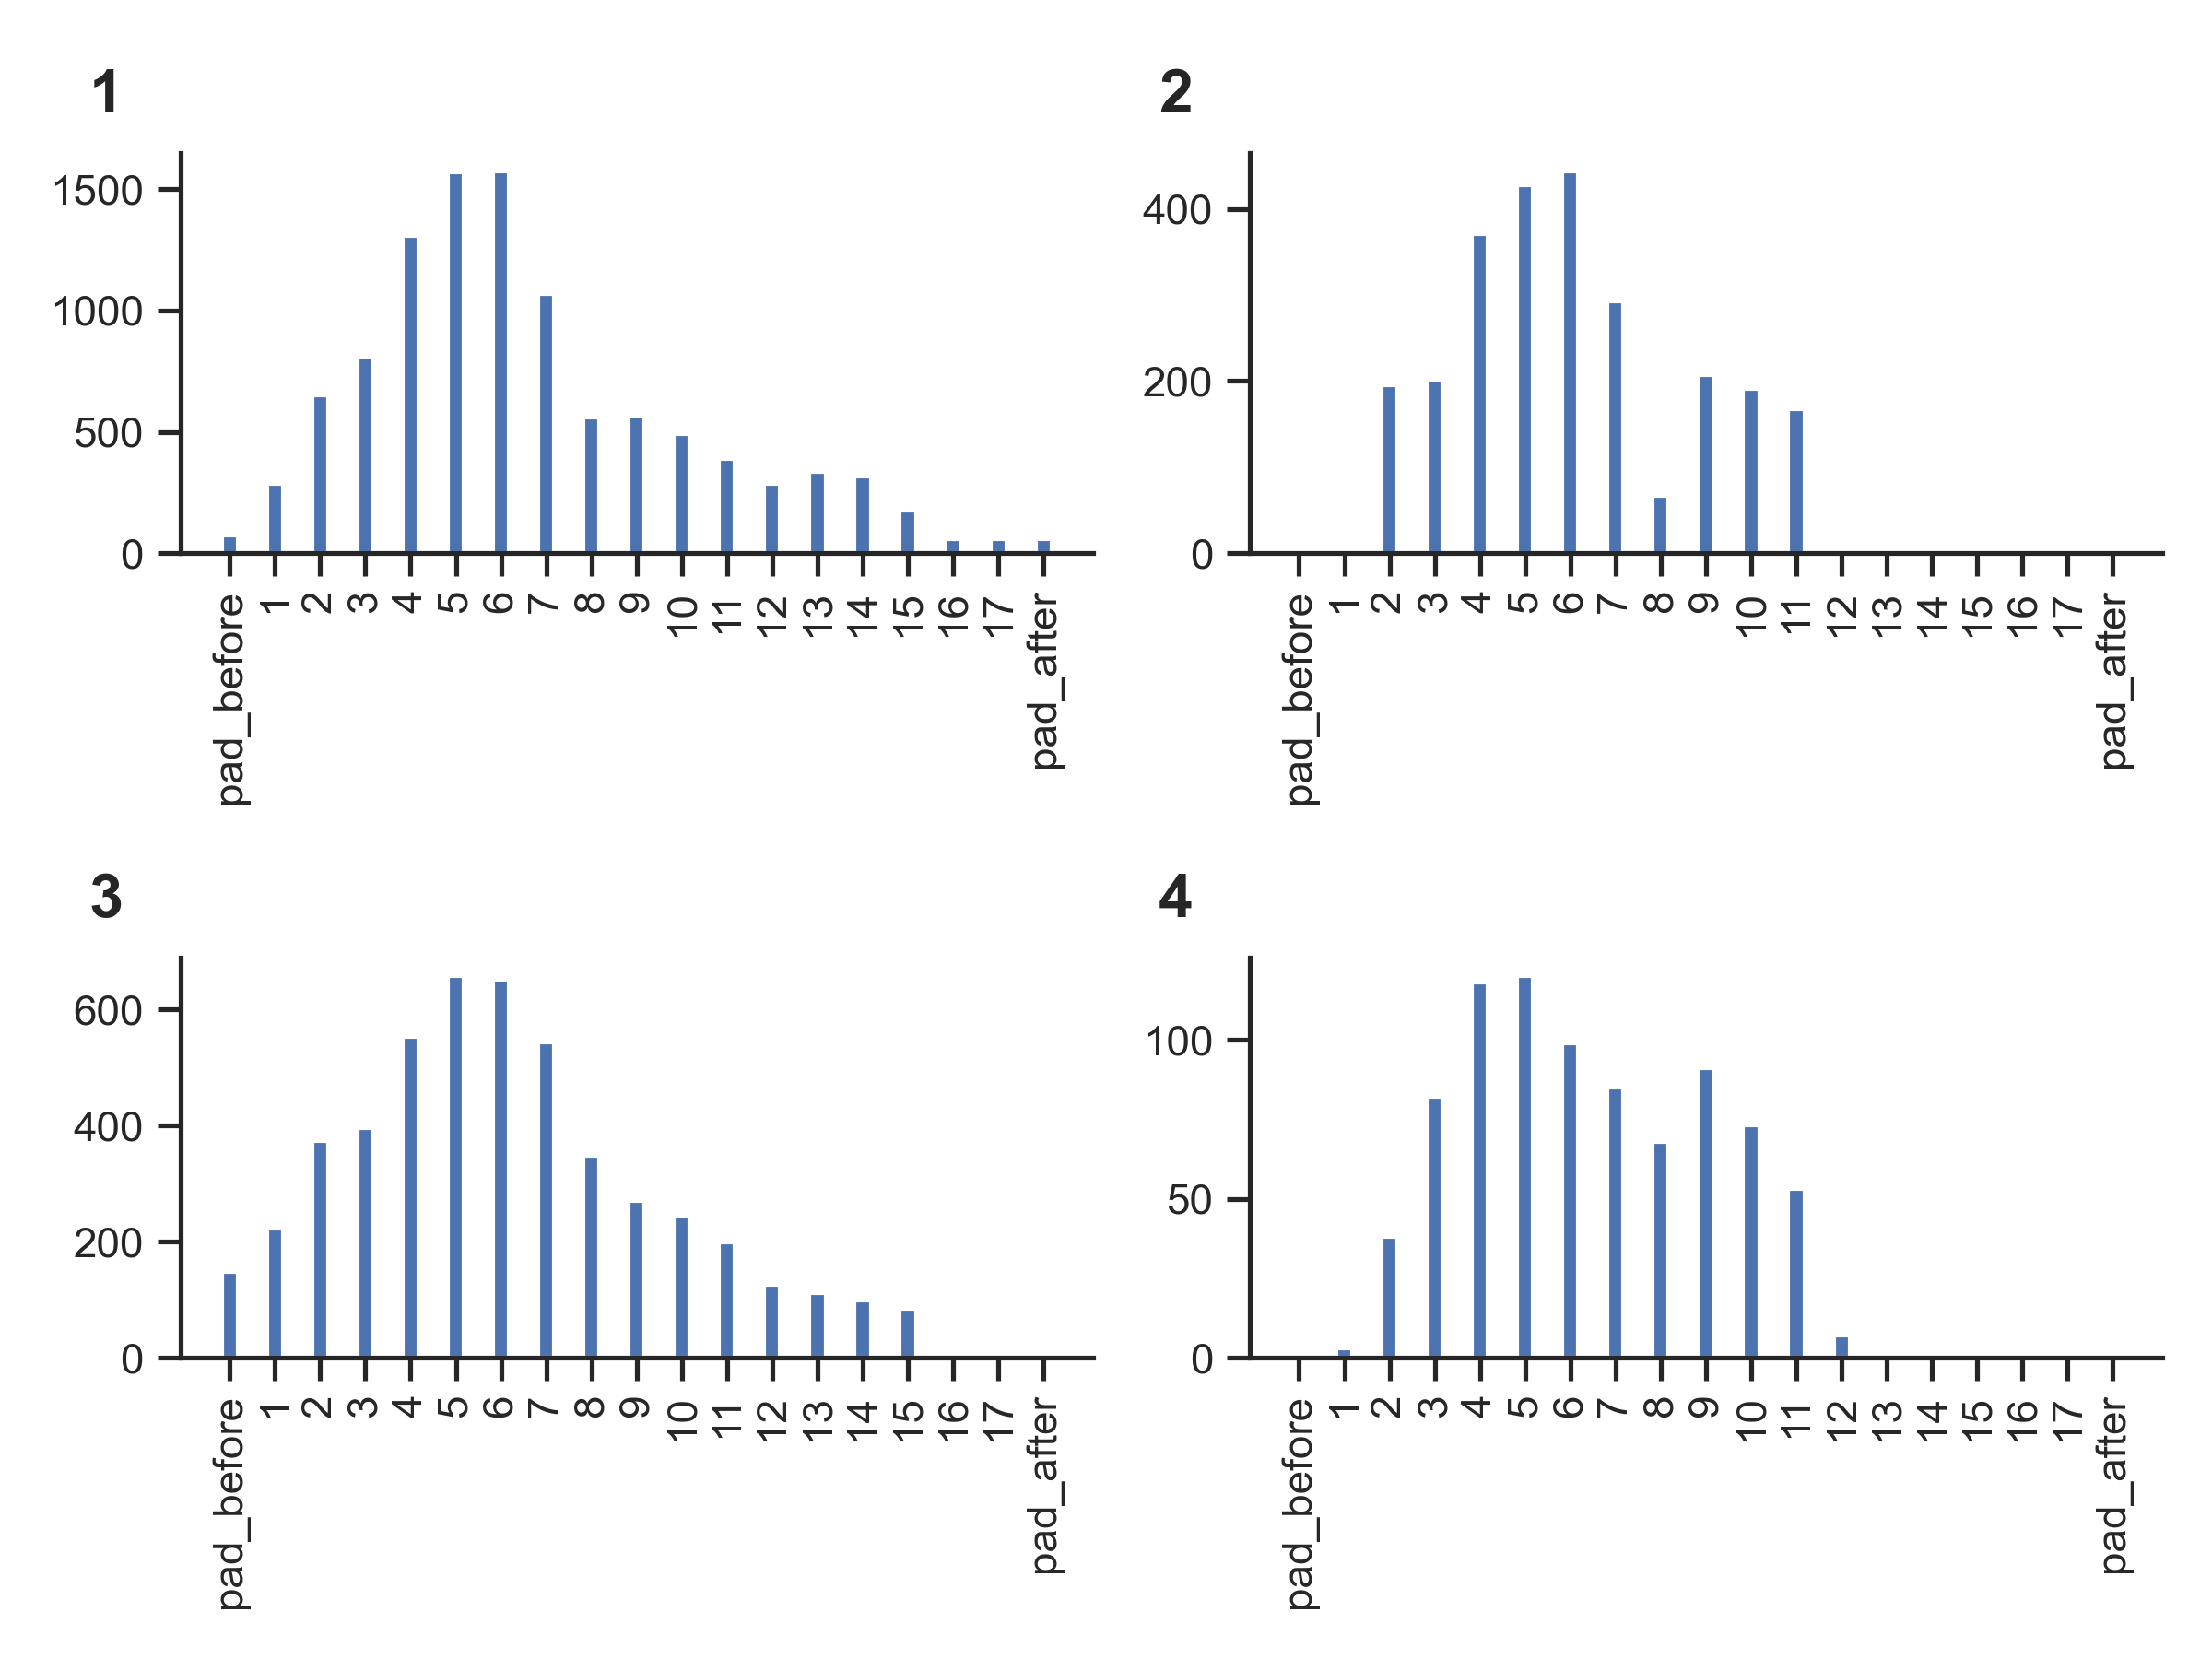
\includegraphics[width=0.95\linewidth]{figures/attention_results/maxpool_cdr3b_gil12.png}
   \caption{Histograms for CDR3{\textbeta}.}
   \label{fig:pool_nlv12b}
\end{subfigure}

\caption{Histograms of number of times a position is selected to contribute information by the maxpooling operation. Positions are determined as contributing if it is used in the convolution selected by maxpooling. \textbf{(1)} Positions selected for CDR3s with positive interaction. \textbf{(2)} Only considering filters with an activation above 0.95 \textbf{(3)} Positions selected for CDR3s with negative interaction. \textbf{(4)} Only considering filters with an activation above 0.95 Data shown for partition held out during training limited to CDR3s with length 12 and specificity for NLV.}
\end{figure}

\newpage
\subsection*{Appendix B - BiLSTM attention for reverse direction}

\begin{figure}[H]
    \centering
    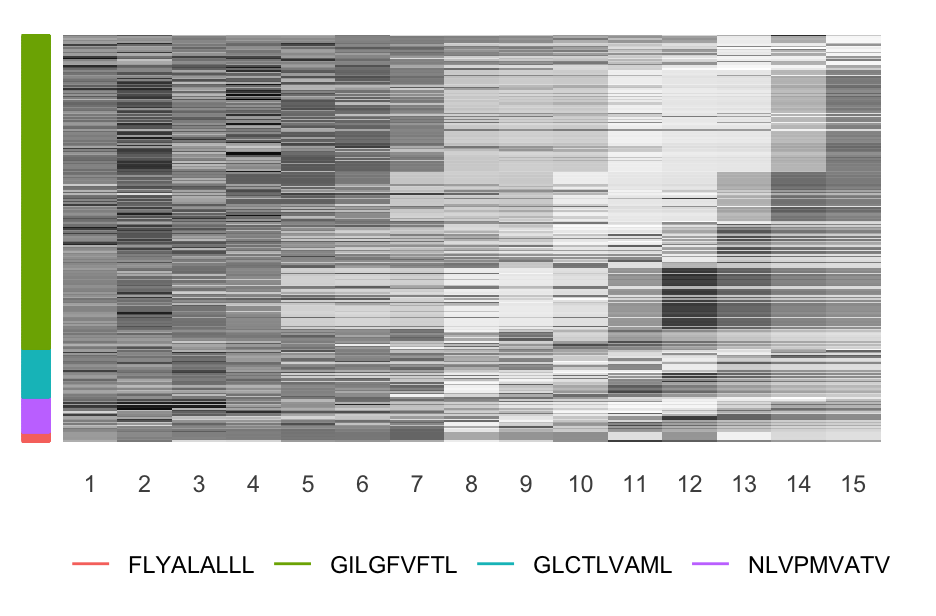
\includegraphics[width=\linewidth]{figures/attention_results/att_cdr3a_r.png}
    \caption{attention on positions for generating the weighted hidden state for the reverse direction of the CDR3{\textalpha}. Sequences have been sorted by CDR length in descending order. Data shown for partition held out during training.}
    \label{fig:att_cdr3a_r}
\end{figure}

\newpage
\subsection*{Appendix C - Sequence logo for GILGFVFTL positive CDR{\textalpha} with length 13 and 11}

\begin{figure}[H]
    \centering
    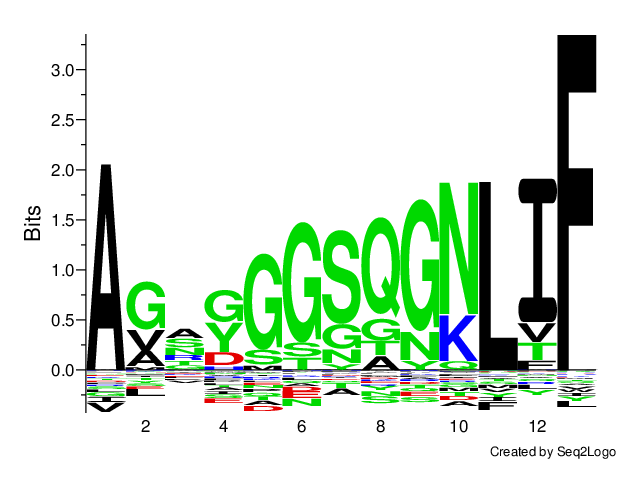
\includegraphics[width=\linewidth]{figures/seq2logo_cd3a_pos_13.png}
    \caption{Logo plot for GILGFVFTL positive CDR3{\textalpha} with a lenght of 13. The sequence contains the same motif as found in \ref{fig:logo_cdr3apos}, but at one position earlier as expected.}
    \label{fig:seq_cdr3a13}
\end{figure}

\begin{figure}[H]
    \centering
    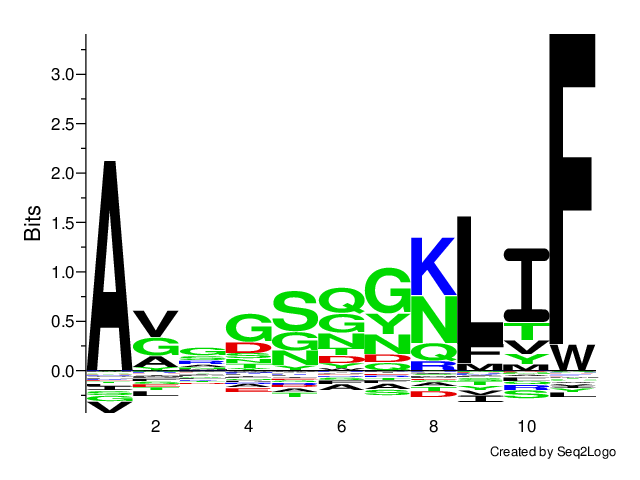
\includegraphics[width=\linewidth]{figures/seq2logo_cd3a_pos_11.png}
    \caption{Logo plot for GILGFVFTL positive CDR3{\textalpha} with a lenght of 11. The sequence contains the same motif as found in \ref{fig:logo_cdr3apos}, but at position 7 and 8.}
    \label{fig:seq_cdr3a11}
\end{figure}